\textit{Solución.} Se implementó el sistema real en Simulink por medio de la ecuación del \hyperref[eq1]{modelo dinámico del proceso}. A continuación se muestra el diagrama de bloques que se obtuvo:

\begin{figure}[!h]
    \centering
    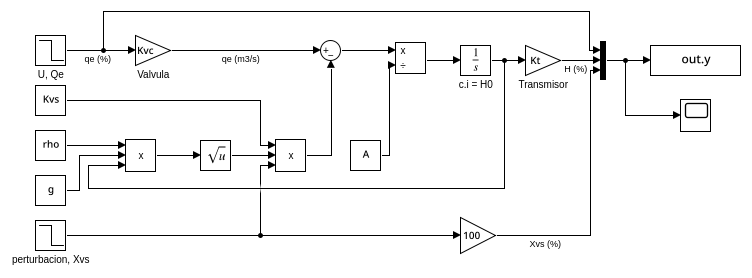
\includegraphics[width = 0.8\linewidth]{figs/fig2.png}
    \caption{Diagrama de bloques del sistema real implementado en Simulink}
    \label{fig2}
\end{figure}

